\section{Introduction}\label{sec:intro}

% \ds{break this long paragraph into smaller ones}
Over the last decade, worst-case optimal join (\WCOJ)
algorithms~\cite{DBLP:conf/pods/NgoPRR12, DBLP:conf/icdt/Veldhuizen14,
  DBLP:journals/sigmod/NgoRR13, DBLP:conf/pods/000118} have emerged as
a breakthrough in one of the most fundamental challenges in query
processing: computing joins efficiently.  Such an algorithm can be
asymptotically faster than traditional binary joins, all the while
remaining simple to understand and
implement~\cite{DBLP:journals/sigmod/NgoRR13}.  These algorithms 
opened up a flourishing field of research, leading to both theoretical
results~\cite{DBLP:journals/sigmod/NgoRR13,DBLP:conf/pods/Khamis0S17}
and practical
implementations~\cite{DBLP:conf/icdt/Veldhuizen14,DBLP:journals/tods/AbergerLTNOR17,DBLP:journals/pvldb/FreitagBSKN20, DBLP:journals/pvldb/MhedhbiS19}.

Over time, a common belief took hold: 
  ``\WCOJ is designed for cyclic queries''.
This belief is rooted in the observation that 
  \WCOJ enjoys lower asymptotic complexity 
  than traditional algorithms for cyclic queries~\cite{DBLP:journals/sigmod/NgoRR13}, 
  but when the query is acyclic, 
  classic algorithms like the Yannakakis algorithm~\cite{DBLP:conf/vldb/Yannakakis81} 
  are already asymptotically optimal. 
Moreover, traditional binary join algorithms have benefited from 
  decades of research and engineering.
Techniques like column-oriented layout, vectorization, 
  and query optimization
  have contributed compounding constant-factor speedups,
  making it challenging for \WCOJ to be competitive in practice.
% \ds{Can you be specific and explain this was done in Hyper}
This has lead many instantiations of \WCOJ,
  including Umbra~\cite{DBLP:journals/pvldb/FreitagBSKN20},
   Emptyheaded~\cite{DBLP:journals/tods/AbergerLTNOR17}, and Graphflow~\cite{DBLP:journals/pvldb/MhedhbiS19},
  to adopt a hybrid approach: 
  using \WCOJ to process parts of the query,
% \rw{Umbra actually does not use \WCOJ only for cycles.
% It relies on the optimizer to detect skew, and use \WCOJ 
%   for skewed joins.}
  and resorting to traditional algorithms (usually binary join) 
  for the rest.
Having two different algorithms in the same system
  requires changing and potentially duplicating existing infrastructure 
  like the query optimizer. 
This introduces complexity, and hinders the adoption of \WCOJ.

The dichotomy of \WCOJ versus binary join has led researchers 
  and practitioners to view the algorithms as opposites.
In this paper, we break down this dichotomy by proposing
  a new framework called \FJ that unifies \WCOJ and binary join.
  % as well as other classic multiway join algorithms.
%
% \rw{The following is not correct. 
%   \FJ can be made equivalent to either binary join or \WCOJ 
%     if we provide a \FJ plan that captures either one. 
%   But we will not execute such a plan.
%   Instead, starting with the original binary plan,
%     we first transform the plan into one that 
%     is neither binary join nor \WCOJ,
%     then execute it with the vectorized algorithm.
%   This is described in the next paragraph as the contributions.}
% \FJ relies on a traditional cost-based optimizer to generate an
%   optimized join tree, then uses a novel execution strategy of the
%   join tree.  Depending on the shape of the query and the join tree,
%   this strategy may be either equivalent to traditional binary index
%   joins, or to a \WCOJ algorithm on a cyclic query.  On standard
%   benchmarks, consisting of acyclic queries, \FJ either matches or
%   outperforms traditional engines.
We propose several new techniques to make \FJ outperform
both binary join and \WCOJ:
% \ds{Have you decided that these are the three main contributions?
%   If we bulletize them then they need to match what we say at the end
%   of the introduction: there we don't mention \COLT but mention
%   experiments.  I suggest that here we remove the bullets and simply
%   list these three contribution sin the text, then at the end of the
%   intro we repeat them in bullets, and add experimental evaluation.
%   Also, the contributions need to align with the text in the paper.}
% \rw{Fixed.}
we design an algorithm to convert any binary join plan to a \FJ plan
that runs as fast or faster; we design a new data structure called
\COLT (for \emph{Column-Oriented Lazy Trie}), adapting the classic
column-oriented layout to improve the trie data structure used in
\WCOJ; and we propose a vectorized execution algorithm for \FJ.

\begin{figure}
    \centering
    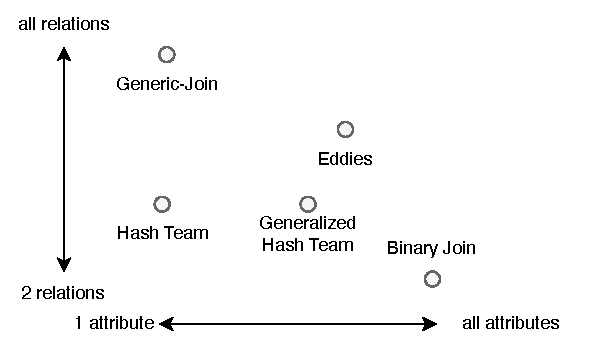
\includegraphics[width=0.55\linewidth]{free-join.pdf}
    \caption{Design space of join algorithms.}
    \label{fig:design-space}
\end{figure}

To explain these contributions we provide some context.
%
In this paper, we focus on algorithms based on hashing,
  and choose \GJ~\cite{DBLP:journals/sigmod/NgoRR13} as a representative of \WCOJ algorithms.
A crucial difference between \GJ and binary join lies 
  in the way they process each join operation. 
Binary join processes two relations at a time, 
  and joins on \emph{all attributes} 
  in the join condition between these two relations. 
In contrast, \GJ processes one attribute at a time, 
  and joins \emph{all relations} that share that attribute.
This suggests a design space of join algorithms, 
  where each join operation may process any 
  number of attributes and relations.
Figure~\ref{fig:design-space} shows this design space
  which also covers classic multiway join algorithms 
  like Hash Team~\cite{DBLP:conf/vldb/GraefeBC98}, 
  Generalized Hash Team~\cite{DBLP:conf/vldb/KemperKW99}
  and Eddies~\cite{DBLP:conf/sigmod/HellersteinA00}.
Being able to join on any number of variables and relations
  frees us from the constraints of all existing algorithms 
  mentioned above. 
% } \yell{I suggest removing the boldface}

Our new framework, \FJ,
  covers the entire design space, 
  thereby generalizing and unifying existing algorithms.
The starting observation is that the execution of a left-deep linear 
  binary join plan is already very similar to \GJ.
While \GJ (reviewed in Sec.~\ref{sec:background}) is traditionally specified as a series of nested loops~\cite{DBLP:journals/sigmod/NgoRR13},
  the push-based model~\cite{DBLP:journals/pvldb/Neumann11,DBLP:journals/pvldb/KerstenLKNPB18} for executing a left-deep linear binary plan
  is also implemented, similarly, as nested loops.
% \rw{Should I add an example of the loop nest, or is that too much detail?}
% \ds{Not here, but please explain this point again in the technical
%   sections, and give an example there.}
The two algorithms also process each join operation similarly:
  each binary hash join iterates over tuples on one relation, 
  and for each tuple probes into the hash table of another relation;
  each loop level in \GJ iterates over the keys of a certain trie,
  and probes into several other tries for each key.
This inspired us to unify hash tables and hash tries into the same data structure, 
  and develop \FJ using iteration and probing as key operations.
This finer-grained view of join algorithms allows \FJ
  to generalize and unify existing algorithms,
  while precisely capturing each of them.

  \FJ takes as input an already optimized binary join plan, and
  converts it into a new kind of plan that we call a \FJ plan.  It
  then optimizes the \FJ plan, resulting in a plan that sits in
  between binary join and \GJ, combining the benefits of both.  On one
  hand \FJ takes full advantage of the design space in
  Figure~\ref{fig:design-space}.  On the other hand, by starting from
  an already optimized binary plan, \FJ takes advantage of existing
  cost-based optimizers; in our system we used binary plans produced by
  the optimizer of DuckDB~\cite{DBLP:conf/cidr/RaasveldtM20,DBLP:conf/vldb/Raasveldt22}.

Next, we address the main source of
  inefficiency in \GJ: the need to construct a trie on each relation
  in the query.  In contrast,  
a binary join plan needs to build a hash map only for each relation 
  on the right-hand side of a join,
  and simply iterates over the relation on the left.
In practice, trie-building has been observed to be a major 
  bottleneck for \GJ~\cite{DBLP:journals/pvldb/MhedhbiS19,DBLP:journals/pvldb/FreitagBSKN20}, 
  making it slower than binary join.
This is because each trie is more expensive to build than a hash map,
  and the left relation is usually chosen to be a large relation 
  by the query optimizer.
One simple optimization in \FJ is that we do not built a trie for
tables that are left children, mimicking the binary plans.
%
However, we go a step further, and introduce the {\em Column-Oriented
  Lazy Trie} (\COLT) data structure, which builds the inner subtries
  lazily, by creating each subtrie on demand.  
We note that this builds on an earlier idea
in~\cite{DBLP:journals/pvldb/FreitagBSKN20}.  As the name suggests,
\COLT adapts the lazy trie data structure
in~\cite{DBLP:journals/pvldb/FreitagBSKN20} to use a column-oriented
layout.  And unlike the original lazy trie which builds at least one
trie level per table, \COLT completely eliminates the cost of trie
building for left tables.


Finally, we describe a method for incorporating vectorized
  processing in \FJ, allowing it to collect multiple data values
  before entering the next iteration level.  
The standard \GJ processes one data value at a time, but, as is the
  case in traditional query engines, this leads to poor cache
  locality.  
Vectorized execution~\cite{DBLP:conf/icde/PadmanabhanAMJ01} was proposed for binary join
  to improve its locality by processing data values in batch.
By breaking down join operations into iterations and probes, 
  \FJ gives rise to a simple vectorized execution algorithm
  that breaks each iteration into chunks and groups together 
  batches of probes.
Our proposal is to our knowledge the first vectorized execution algorithm for \GJ.

We implemented \FJ as a standalone Rust library, and
compared it with two baselines:
  \begin{enumerate*}
    \item our own \GJ implementation in Rust, and
    \item the binary hash join implemented in
      DuckDB~\cite{DBLP:conf/cidr/RaasveldtM20,DBLP:conf/vldb/Raasveldt22},
      a state-of-the-art in-memory database.
    \end{enumerate*}
    %%%%%%%%%% No need for experimental details here, just some highlights
%%%   We conduct experiments on the popular Join Order
%%%   Benchmark~\cite{DBLP:journals/pvldb/LeisGMBK015} and the
%%%   LSQB~\cite{} benchmark.
  We found that, on acyclic queries, \FJ is up to \imdbmaxfjbj
  faster than binary join, and up to \imdbmaxfjgj faster than \GJ; on
  cyclic queries, \FJ is up to 15.45x faster than binary join, and up
  to 4.08x faster than \GJ.
  % \FJ also retains its advantage even when the optimizer chooses a poor plan.
%%%   We conduct additional experiments on
%%%   synthetic data for star and chain queries, as well as ablation
%%%   studies on the optimizations.  Finally, we compare \FJ and binary
%%%   hash join on their robustness against bad query plans.  Given a bad
%%%   query plan, \FJ runs up to \hjbad and \gjbad faster than binary join
%%%   and \GJ, respectively.

  While optimizers for binary plans have been developed and improved
  over decades~\cite{DBLP:conf/sigmod/SelingerACLP79}, little
  is known about optimizing \GJ.  A \GJ plan consists of a total order
  on its variables, and its run time does depend on the choice of this
  order.  But since the theoretical analysis of \GJ guarantees worst
  case optimality for {\em any} variable order, it is a folklore
  belief that \GJ is more robust than binary join plans to poor
  choices of the optimizer.  We also conduced experiments measuring
  the robustness of the three types of plans (binary, \GJ, \FJ) to
  poor choices of the optimizer.  We found that \GJ is indeed the
  least sensitive, while \FJ, like binary joins, suffers more from the
  poor optimization choices of the optimizer, since both rely on a
  cost-based optimized plan.  However, \GJ starts from worse baseline
  than \FJ.  In other words, \FJ takes better advantage of a good
  plan, when available, than \GJ does.


  
In summary, we make the following contributions in this paper:
% \ds{Please reference the sections where these contributions are
%   described.  Currently the do NOT align with the contributions
%   mentioned earlier and discussed in the introduction.  This needs to
%   be fixed.}
% \rw{Fixed.}
\begin{enumerate}
  \item \FJ, a framework unifying existing join algorithms (Section~\ref{sec:free-join}).
  \item An algorithm to converting any binary join plan into an
    optimized \FJ plan (Section~\ref{sec:bj-to-fj}).
  \item \COLT, a column-oriented lazy trie data structure (Section~\ref{sec:colt}).
  \item A vectorized execution algorithm for \FJ (Section~\ref{sec:vectorized-execution}).
  \item Experiments evaluating the algorithms and optimizations (Section~\ref{sec:eval}).
\end{enumerate}